\chapter{Introduction}
\label{sec:intro}

Single molecule force spectroscopy (SMFS) is the study of folding and
unfolding transitions in proteins under tension.  By measuring these
transitions, we hope to gain insight into fundamental protein
behavior.  SMFS is an attempt to bridge the gap between chemists
studying folding and unfolding kinetics in bulk solutions and
theorists simulating protein behavior at the amino-acid level.  An
increased understanding of protein folding would guide researchers in
developing drugs targeting biologically significant receptors and
enzymes.  In this chapter, I describe the protein folding problem in a
general sense (\cref{sec:folding-problem}), discuss theoretical
frameworks for understanding protein folding
(\cref{sec:energy-landscape}), highlight the role of SMFS in extending
this understanding (\cref{sec:single-molecule}), and explain the role
of unfolding experiments in understanding protein folding
(\cref{sec:unfolding}).  The last section in this chapter gives a
roadmap for the rest of the thesis (\cref{sec:outline}).

\section{The protein folding problem}
\label{sec:folding-problem}

% Why study protein folding?
In biological systems the most important molecules, such as proteins,
nucleic acids, and polysaccharides, are all polymers.  Understanding
the properties and functions of these polymeric molecules is crucial
in understanding the molecular mechanisms behind structures and
processes in cells.

% What do genes do?  Why is protein folding interesting?
An organism's genetic code is stored in DNA in the cell nucleus.
DNA sequencing is a fairly well developed field, with fundamental work
such as the Human Genome Project seeing major development in the early
2000s\citep{wolfsberg01,mcpherson01,collins03}.  It is estimated that
human genetic information contains approximately 25,000 genes, each
encoding a protein\citep{claverie01,venter01}.  Knowing the amino acid
sequence for a particular protein, however, does not immediately shed
light on the protein's role in the body, or even the protein's
probable conformation.  Indeed, a protein's conformation is often
vitally important in executing its biological tasks
(\cref{fig:ligand-receptor}).  Unfortunately predicting a protein's
stable conformations from it's amino acid sequence has proven to be
remarkably difficult, as has the inverse problem of finding sequences
that form a given conformation.
%
\nomenclature[text ]{DNA}{Deoxyribonucleic acid.}

\begin{figure}
  \begin{center}
  \includegraphics[width=2in]{figures/biotin-streptavidin/1SWE}%
  \caption{Complex of biotin\index{biotin} (red) and a
    streptavidin\index{streptavidin} tetramer (green)
    (\href{http://dx.doi.org/10.2210/pdb1swe/pdb}{PDB ID: 1SWE})%
    \citep{freitag97}.  The correct streptavidin conformation creates
    the biotin-specific binding pockets.  Biotin-streptavidin is a
    model ligand-receptor pair isolated from the bacterium
    \species{Streptomyces avidinii}%
    \index{Streptomyces@\species{Streptomyces avidnii}}.  Streptavidin
    binds to cell surfaces, and bound biotin increases streptavidin's
    cell-binding affinity\citep{alon90}.  Figure generated with
    \citetalias{pymol}.
    \label{fig:ligand-receptor}}
  \end{center}
\end{figure}


\section{Protein folding energy landscapes}
\label{sec:energy-landscape}

% the free energy landscape
Finding a protein's lowest energy state via a brute force sampling of
all possible conformations is impossibly inefficient, due to the
exponential scaling of possible conformations with protein length, as
outlined by \citet{levinthal69}.  This has lead to a succession of
models explaining the folding mechanism.  For a number of years, the
``pathway'' model of protein folding enjoyed popularity
(\cref{fig:folding:pathway})\citep{levinthal69}.  More recently, the
``landscape'' or ``funnel'' model has come to the fore
(\cref{fig:folding:landscape})\citep{dill97}.  Both of these models
reduce the conformation space to a more approachable analog, and their
success depends on striking a useful balance between simplicity and
accuracy.

\begin{figure}
  \begin{center}
  \subfloat[][]{
    \begin{tikzpicture}[->,node distance=1.5cm]
      \tikzstyle{every state}=[draw=white]
      \node[state] (U)                 {$U$};
      \node[state] (I1)  [right of=U]  {$I_1$};
      \node[state] (I1X) [below of=I1] {$I_1^X$};
      \node[state] (I2)  [right of=I1] {$I_2$};
      \node[state] (I2X) [below of=I2] {$I_2^X$};
      \node[state] (N)   [right of=I2] {$N$};
    
      \path[<->] (U)  edge (I1)
                 (I1) edge (I1X)
                 (I1) edge (I2)
                 (I2) edge (I2X)
                 (I2) edge (N);
    \end{tikzpicture}\label{fig:folding:pathway}}
  % \hspace{.25in}%
  \subfloat[][]{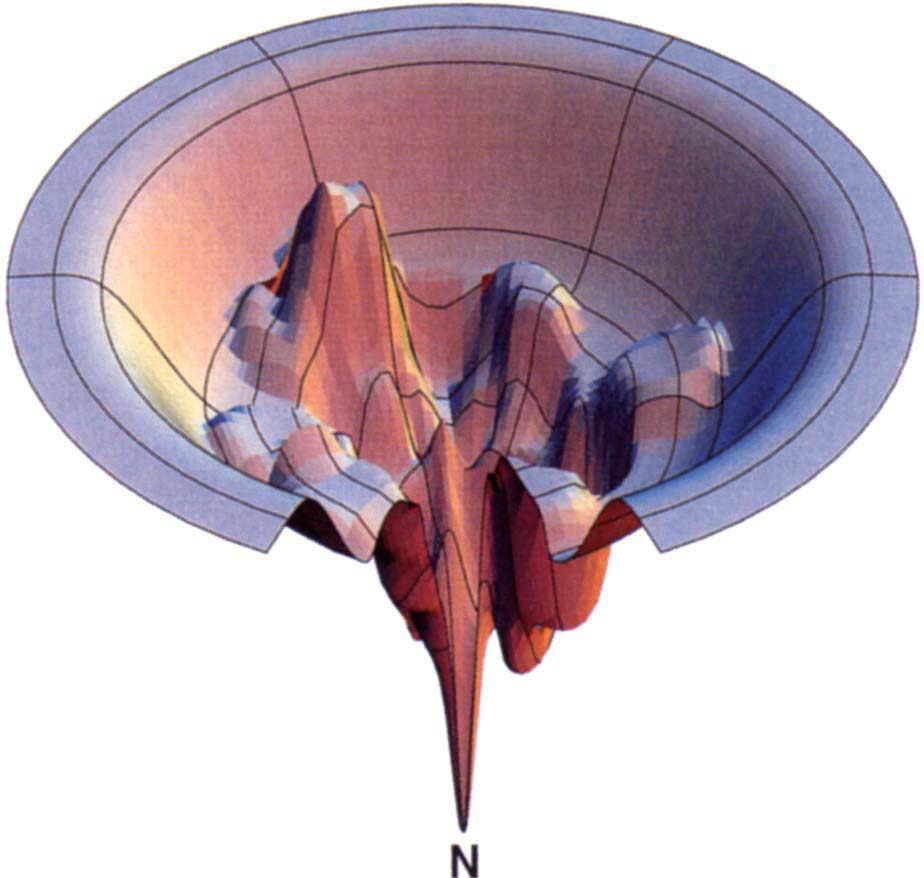
\includegraphics[width=2in]{figures/schematic/dill97-fig4}%
    \label{fig:folding:landscape}}
  \caption{\protect\subref{fig:folding:pathway} A ``double T'' example
    of the pathway model of protein folding, in which the protein
    proceeds from the native state $N$ to the unfolded state $U$ via a
    series of metastable transition states $I_1$ and $I_2$ with two
    ``dead end'' states $I_1^X$ and $I_2^X$.  Adapted from
    \citet{bedard08}.
    \protect\subref{fig:folding:landscape} The landscape model of
    protein folding, in which the protein diffuses through a
    multi-dimensional free energy landscape.  Separate folding
    attempts may take many distinct routes through this landscape on
    the way to the folded state.  Reproduced from
    \citet{dill97}.\label{fig:folding}}
  \end{center}
\end{figure}

When the choice of theoretical approach becomes murky, you must gather
experimental data to help distinguish between similar models.
Separating the pathway model from the funnel model is only marginally
within the realm of current experimental techniques, but with higher
throughput and increased automation it should be easier to make such
distinctions in the near future.


\section{Why \emph{single} molecule?}
\label{sec:single-molecule}

The large size of proteins relative to simpler molecules limits the
information attainable from bulk measurements, because the
macromolecules in a population can have diverse conformations and
behaviors.  Bulk measurements average over these differences,
producing excellent statistics for the mean, but making it difficult
to understand the variation.  The individualized, and sometimes rare,
behaviors of macromolecules can have important implications for their
functions inside the cell.  Single molecule techniques, in which the
macromolecules are studied one at a time, allow direct access to the
variation within the population without averaging.  This provides
important and complementary information about the functional
mechanisms of several biological systems\citep{bustamante08}.

Single molecule techniques provide an opportunity to study protein
folding and unfolding at the level of a single molecule, where the
distinction between the pathway model and funnel model is clearer.
They also provide a convenient benchmark for verifying molecular
dynamics simulations, because it takes lots of computing power to
simulate even one biopolymer with anything close to atomic resolution
over experimental time scales.  Even with significant computing
resources, comparing molecular dynamics results with experimental data
remains elusive.  For example, experimental pulling speeds are on the
order of \bareU{$\mu$m/s}, while simulation pulling speeds are on the
order of \bareU{m/s}\citep{lu98,lu99,rief02,zhao06,berkemeier11}.

% why AFM & what an AFM is
Single molecule techniques for manipulating biopolymers include
optical measurements, \ie, single molecule fluorescence microscopy and
spectroscopy, and mechanical manipulations of individual
macromolecules, \ie, force microscopy and spectroscopy using atomic
force microscopes (AFMs), laser tweezers\citep{kellermayer97,forde02},
magnetic tweezers\citep{smith92}, biomembrane force
probes\citep{merkel99}, and centrifugal
microscopes\citep{halvorsen09}.  These techniques cover a wide range
of approaches, and even when the basic approach is the same
(e.g.\ force microscopy), the different techniques span orders of
magnitude in the range of their controllable parameters.
%
\nomenclature[text ]{AFM}{Atomic force microscope (or microscopy).}

\section{Why \emph{un}folding?}
\label{sec:unfolding}

There's a lot of talk about protein \emph{folding} in this chapter,
while the rest of the thesis (and the title) are about
\emph{unfolding}.  If you understand protein folding, you can use your
understanding to design drugs with a particular conformation, or
predict the conformation of a biologically important receptor
(\cref{sec:folding-problem}).  Understanding protein unfolding is less
directly useful, because unfolded proteins are rarely biologically
relevant (although it does happen\citep{dyson05}).

The focus on unfolding is mainly because it's easier to unravel
proteins by pulling on their ends (\cref{sec:procedure}) than it is to
fold them into their native state by pushing on those ends
(\cref{fig:ligand-receptor,fig:I27}).  For proteins with smooth enough
energy landscapes, the folding and unfolding routes will be similar,
so knowledge about the unfolding behavior \emph{does} shed light on
the folding behavior.

Practically, the distinction between folding and unfolding makes
little difference, because drug designers and doctors are not
consuming SMFS results directly.  For researchers calibrating
molecular dynamics simulations, it doesn't matter if you compare
simulated folding experiments with experimental folding experiments,
or simulated unfolding experiments with experimental unfolding
experiments.  The important thing is to compare your simulation
against \emph{some} experimental benchmarks.  If your molecular
dynamics simulation successfully predicts a protein's unfolding
behavior, it makes me more confident that it will correctly predict
the protein's native folding behavior.


\section{Thesis outline}
\label{sec:outline}

\Cref{sec:methods} of this thesis outlines the apparatus and methods
for single molecule force spectroscopy with an atomic force
microscope.  \Cref{sec:sawsim} presents my \sawsim\ Monte Carlo
simulation for modeling unfolding/refolding behavior.  By comparing
model simulations with experimental measurements, we can gain insight
into the protein's kinetics.  After \cref{sec:sawsim}, you should have
a pretty firm grasp of the underlying physics, so we'll move on to
\cref{sec:pyafm} and discuss my \pyafm\ and \unfoldprotein\ experiment
control software.  With both the kinetic theory and procedure taken
care of, \cref{sec:calibcant} discusses thermal cantilever
calibration, deriving the theoretical approach and presenting my
\calibcant\ automatic calibration software.

Moving away from experiment control, \cref{sec:hooke} presents the
\Hooke\ suite for extracting unfolding force histograms (for
comparison with \sawsim\ simulations).  In \cref{sec:salt}, I pull all
the pieces together (experiment control, post processing, and
simulation) to carry out unfolding experiments on the
immunoglobulin-like domain 27 from human Titin (I27) in buffers with
different ionic strength.  We close with \cref{sec:future}, which
summarizes my conclusions and discusses possible directions for future
work.
